\documentclass{article}
\usepackage[utf8]{inputenc}
\usepackage[english]{babel}
\usepackage{graphicx}
\usepackage{siunitx}
\usepackage{listings}
\usepackage{color}
\usepackage[toc,page]{appendix}
\renewcommand{\appendixtocname}{Přílohy}
\renewcommand{\appendixpagename}{Přílohy}

\definecolor{mygreen}{rgb}{0,0.6,0}
\definecolor{mygray}{rgb}{0.5,0.5,0.5}
\definecolor{mymauve}{rgb}{0.58,0,0.82}

\lstset{
    language=SQL,
    keywordstyle=\color{blue},
    numbers=left,
    numbersep=5pt,
    numberstyle=\tiny\color{mygray},
    commentstyle=\color{mygreen},
    morekeywords={*, REPLACE, WITH, FUNCTION, RETURNS, BODY, DECLARE, RECORD, BEGIN, CONTINUE, PERFORM, RAISE NOTICE, NEW},
    stringstyle=\color{mymauve},
    breaklines=true,
    tabsize=2,
}
\lstset{literate=
  {á}{{\'a}}1 {é}{{\'e}}1 {í}{{\'i}}1 {ó}{{\'o}}1 {ú}{{\'u}}1
  {Á}{{\'A}}1 {É}{{\'E}}1 {Í}{{\'I}}1 {Ó}{{\'O}}1 {Ú}{{\'U}}1
  {à}{{\`a}}1 {è}{{\`e}}1 {ì}{{\`i}}1 {ò}{{\`o}}1 {ù}{{\`u}}1
  {À}{{\`A}}1 {È}{{\'E}}1 {Ì}{{\`I}}1 {Ò}{{\`O}}1 {Ù}{{\`U}}1
  {ä}{{\"a}}1 {ë}{{\"e}}1 {ï}{{\"i}}1 {ö}{{\"o}}1 {ü}{{\"u}}1
  {Ä}{{\"A}}1 {Ë}{{\"E}}1 {Ï}{{\"I}}1 {Ö}{{\"O}}1 {Ü}{{\"U}}1
  {â}{{\^a}}1 {ê}{{\^e}}1 {î}{{\^i}}1 {ô}{{\^o}}1 {û}{{\^u}}1
  {Â}{{\^A}}1 {Ê}{{\^E}}1 {Î}{{\^I}}1 {Ô}{{\^O}}1 {Û}{{\^U}}1
  {œ}{{\oe}}1 {Œ}{{\OE}}1 {æ}{{\ae}}1 {Æ}{{\AE}}1 {ß}{{\ss}}1
  {ű}{{\H{u}}}1 {Ű}{{\H{U}}}1 {ő}{{\H{o}}}1 {Ő}{{\H{O}}}1
  {ç}{{\c c}}1 {Ç}{{\c C}}1 {ø}{{\o}}1 {å}{{\r a}}1 {Å}{{\r A}}1
  {€}{{\euro}}1 {£}{{\pounds}}1 {«}{{\guillemotleft}}1
  {»}{{\guillemotright}}1 {ñ}{{\~n}}1 {Ñ}{{\~N}}1 {¿}{{?`}}1
}

\rmfamily

\begin{document}

\begin{titlepage}
		
\includegraphics[width=300px]{fav_logo.pdf}\par
		\vspace{1cm}
		\centering
		{\scshape\LARGE Západočeská univerzita \par}
		\vspace{0.5cm}
		{\scshape\Large Fakulta aplikovaných věd \par}
		\vspace{2cm}
		{\Large\bfseries Semestrální práce předmětu KIV/DB2 \par}
		\vspace{0.5cm}
		{\Large Hledání min \par}
		\vspace{0.5cm}
		{\Large\itshape Petr Štechmüller\par}
		\vfill
		{\large \today\par}
\end{titlepage}

\tableofcontents

\section{Zadání}
Cílem této práce je navrhnout a vytvořit relační databázi pro hraní známé počítačové hry Hledání min. 
Protože bude řešena pouze databázová vrstva aplikace, 
snažte se co nejvíce programových rutin uložit do databáze 
a také zajistěte jejich automatickou aktivaci při nastalé události. 

Herní oblast má zpravidla tvar obdélníku, ve kterém se nachází několik min. 
Velikost oblasti a počet min v ní definuje obtížnost hry. 
Hráč si může vybrat jednu ze tří předdefinovaných obtížností nebo si může definovat obtížnost vlastní. 
Úkolem hráče je odkrýt všechna pole oblasti, která nejsou zaminována. 
Hráči se bude od začátku hry měřit čas, aby bylo možné dosažené výsledky porovnávat. 
Po odkrytí libovolného pole (hráčem nebo databází) může
nastat jedna z těchto událostí:
\begin{itemize}
    \item Hráč šlápl na minu. Hra končí neúspěchem a výsledek se zaznamená do databáze.
    \item Bylo odkryto poslední pole, na kterém není mina. Hra končí úspěchem, protože zbylá
neodkrytá pole obsahují miny. Také v tomto případě se výsledek uloží do databáze.
    \item Bylo odkryto pole, které je volné a nesousedí s žádným zaminovaným polem. V tomto
případě databáze automaticky odkryje všechna sousední pole – ty mají společný min.
jeden vrchol.
\end{itemize}

Pro snazší hraní si může hráč označovat ta pole, o kterých si myslí, že jsou zaminovaná.
K tomuto rozhodnutí mu pomohou čísla již odkrytých polí, která určují, s kolika zaminovanými
poli toto pole sousedí. Takto označené pole nelze odkrýt, ale toto označení lze kdykoliv zrušit.

\subsection{Tabulky}
{\renewcommand\labelitemi{}
\begin{itemize}

    \item \textit{OBTIZNOST} - Každá hra musí mít definovanou obtížnost. Buď bude vybrána předdefinovaná,
        nebo si hráč definuje obtížnost vlastní. Hodnoty parametrů vlastní obtížnosti se
        ukládají do tabulky \textit{OBLAST}. Podle originální hry jsou předdefinované
        obtížnosti nastaveny takto:
        \begin{itemize}
            \item Začátečník: 9 řádků x 9 sloupců, 10 min
            \item Pokročilý: 16 řádků x 16 sloupců, 40 min
            \item Expert: 16 řádků x 30 sloupců, 99 min
        \end{itemize}
    
    \item \textit{OMEZENI} - Každá vlastní obtížnost musí splňovat jistá     
        omezení. Např. počet řádků či sloupců nesmí být menší než 9 a větší než 
        100. Také je vhodné pohlídat, aby
        počet rozmístěných min v zaminované oblasti nebyl příliš velký, např.
        nepřekročil 40 procent její velikosti.
    
    \item \textit{OBLAST} - Každá zaminovaná oblast je vytvořená podle vlastní 
        obtížnosti  a obsahuje její hodnoty. 
        Hráč má za úkol oblast od min vyčistit.
    
    \item \textit{POLE} - Elementární část zaminované oblasti definovaná svými 
        souřadnicemi, která může nést minu nebo informaci, 
        s kolika zaminovanými poli sousedí.
    
    \item \textit{MINA}-  Hráčem označovaná pole, o kterých si myslí, že jsou 
        zaminovaná.
    
    \item \textit{TAH}-  Hráčem odkrývaná pole v zaminované oblasti. 
        Ke každému tahu se bude automaticky ukládat časová značka, 
        kdy byl tah vykonán.
    
    \item \textit{STAV} - Číselník obsahující, v jakých stavech se hra 
        může vyskytovat. Stavy mohou být tyto: 
        \begin{itemize}
            \item rozehraná
            \item úspěšně ukončení
            \item neúspěšně ukončená
        \end{itemize}
    
    \item \textit{HRA} - Průběžně aktualizované informace o probíhající hře. Obsahuje časové značky
    prvního a naposledy provedeného tahu, počet označených min a stav hry.
\end{itemize}
}
\subsection{Pohledy}
{\renewcommand\labelitemi{}
\begin{itemize}
    \item \textit{CHYBNE\_MINY} - Seznam polí v zaminované oblasti, které byly     chybně označené jako
        zaminované. Nabízí data pro všechny oblasti.
    
    \item \textit{VITEZOVE} - Výsledková tabulka her, které byly úspěšně 
        dokončené. Měla by ukazovat parametry obtížnosti (rozměry oblasti 
        a počet min) dané hry a také dobu hraní hry (rozdíl časových značek 
        posledního a prvního tahu).
    
    \item \textit{PORAZENI} - Výsledková tabulka her, které byly neúspěšně 
        dokončené. Měla by navíc
        (oproti pohledu \textit{VITEZOVE}) ukazovat, 
        kolik min bylo správně odhaleno.
    
    \item \textit{OBLAST\_TISK} - Zobrazení celé zaminované oblasti včetně 
        odkrytých polí a (hráčem) označených min. 
        Každý řádek oblasti bude zobrazen voláním funkce 
        \textit{RADEK\_OBLASTI}.
\end{itemize}
}

\subsection{Procedury}
{\renewcommand\labelitemi{}
\begin{itemize}
    \item \textit{ZAMINUJ\_OBLAST} - Položení min na (náhodná) místa v definované oblasti. Počet
    zaminovaných polí je uloženo v tabulce \textit{OBLAST}. Do tabulky POLE
    ukládá hodnotu -1.
    
    \item \textit{SPOCITEJ\_OBLAST} - Pro každé nezaminované pole v oblasti spočítá, s kolika zaminovanými
    poli sousedí. Do tabulky \textit{POLE} ukládá hodnoty z intervalu 0 až 8.
    
    \item \textit{ODKRYJ\_POLE} - Rekurzivní procedura, která pro právě odkryté pole, které nesousedí
    s žádným zaminovaným polem, odkryje všechna jeho neodkrytá
    sousední pole.
    
    \item \textit{OZNAC\_MINY} - Po úspěšném dohrání hry budou dosud neodkrytá pole označená jako
    zaminovaná, tj. vloží odpovídající záznamy do tabulky MINA.
\end{itemize}
}

\subsection{Funkce}
{\renewcommand\labelitemi{}
\begin{itemize}
    \item \textit{SPATNY\_PARAMETR} - Oznámí, zda hodnota parametru vlastní obtížnosti porušila definovaná
    omezení.
    
    \item \textit{RADEK\_OBLASTI} - Vrátí řetězec znaků ukazující aktuální podobu daného řádku
    zaminované oblasti.
    
    \item \textit{ODKRYTA\_MINA} - Oznámí, že právě odkryté pole skrývá minu, což znamená neúspěšný
    konec hry.
    
    \item \textit{MNOHO\_MIN} - Nelze označit více zaminovaných polí, než kolik min je v oblasti.
    
    \item \textit{VYHRA} - Počet neodkrytých polí se rovná počtu min, které se v oblasti nachází.
    Pokud ano, hra končí úspěchem.
\end{itemize}
}

\subsection{Triggery}
O automatickou činnost v databázi se budou starat triggery, především o:
\begin{itemize}
    \item hlídání hodnot parametrů vlastní obtížnosti (volání funkce \textit{SPATNY\_PARAMETR}).
    \item kopírování hodnot parametrů obtížnosti pro aktuální oblast, pokud byla zvolena základní obtížnost.
    \item zaminování nastavené oblasti (volání procedury \textit{ZAMINUJ\_OBLAST}) 
        a očíslování polí této oblasti (volání procedury \textit{SPOCITEJ\_OBLAST}).
    \item volání automatických kontrol (volání funkcí \textit{ODKRYTA\_MINA} a \textit{VYHRA}) 
        a případně akcí (volání procedury \textit{ODKRYJ\_POLE}) při odkrytí pole.
    \item zabránění odkrytí již odkrytého pole.
    \item hlídání počtu polí označených jako zaminované (volání funkce \textit{MNOHO\_MIN}).
    \item zabránění označení pole jako zaminované, které je již takto označeno nebo je odkryté.
    \item průběžnou aktualizaci hry po každém jejím tahu.
    \item označení min, pokud hra skončila úspěšně (volání procedury \textit{OZNAC\_MINY}).
    \item zabránění odkrytí pole, pokud hra (neúspěšně) skončila.
    \item zabránění odkrytí pole, které je hráčem označené jako zaminované.
\end{itemize}

\subsection{Konfigurace a průběh hry}
\begin{enumerate}
    \item Jednorázová konfigurace databáze:
    \begin{itemize}
        \item Naplnění tabulky \textit{OBTIZNOST} daty reprezentující 3 základní obtížnosti hry.
        \item Naplnění tabulky \textit{OMEZENI} daty definující omezení pro vlastní obtížnost hry.
        \item Naplnění tabulky \textit{STAV} daty odpovídající různým stavům hry
    \end{itemize}
    \item Hra je zahájena vložením nového záznamu do tabulky \textit{OBLAST}. Automaticky se spustí
        plnění daty tabulky \textit{POLE}, které reprezentují podobu definované zaminované oblasti.
        Nakonec se do tabulky \textit{HRA} automaticky vloží nový záznam.
    \item Dále má hráč na výběr jednu z možností:
    \begin{itemize}
        \item Zobrazit si aktuální podobu zaminované oblasti prostřednictvím pohledu
        \textit{OBLAST\_TISK}.
        \item Odkrýt libovolné pole vložením záznamu do tabulky \textit{TAH}. Dále dochází
            k aktualizaci příslušného záznamu v tabulce \textit{HRA}.
        \item Označit libovolného pole jako mina vložením záznamu do tabulky \textit{MINA}.
        \item Zrušit označení zaminovaného pole smazáním odpovídajícího záznamu
            v tabulce \textit{MINA}.
    \end{itemize}
    \item Pokud hra pokračuje, pokračuj bodem 3, jinak bodem 5 (úspěch) nebo 6 (neúspěch).
    \item Hra skončila úspěchem. Je vhodné si zobrazit:
        \begin{itemize}
            \item Výsledkovou listinu vítězů voláním pohledu \textit{VITEZOVE}.
            \item Zobrazení odminované oblasti voláním pohledu \textit{OBLAST\_TISK}.
        \end{itemize}
    \item Hra skončila neúspěchem. Je vhodné si zobrazit:
        \begin{itemize}
            \item Výsledkovou listinu poražených voláním pohledu \textit{PORAZENI}.
            \item Seznam chybně označených min voláním pohledu \textit{CHYBNE\_MINY}.
        \end{itemize}
    \item Novou hru zahájíme bodem 2.
        
\end{enumerate}


\section{Datová analýza}
Datový model databáze jsem přesně zachoval podle zadání.
V příloze \ref{fig:era} je vidět ERA model databáze.


\section{Funkční analýza}
V této sekci budu demonstrovat zajímavé části kódu.
První ukázka kódu \ref{lst:vitezove} obsahuje kód pro pohled s vítěznými hrami.
V pohledu zobrazuji sloupečky: id hry, id oblasti, doba hrani, počet řádků, počet sloupců,
celkový počet min a obtížnost. Doba hraní se vypočítá jako rozdíl mezi prvním
a posledním tahem. To jsem realizoval pomocí rozdílu dvou SELECTů.

\begin{minipage}{\linewidth}
\lstinputlisting[language=SQL, caption={Pohled Vítězové}, label={lst:vitezove}]{code/vitezove.sql}
\end{minipage}


Druhá ukázka pohledu \ref{lst:chybne_miny} se zaměřuje na kód pro zobrazení chybně označených min.
Rozhodl jsem se, že chybné miny se budou zobrazovat pouze u her, které již byly neúspěšně
dohrány. To zajišťuje podmínka \lstinline{hra.id_stav = 3}.

\begin{minipage}{\linewidth}
\lstinputlisting[language=SQL, caption={Pohled Chybné miny}, label={lst:chybne_miny}]{code/chybne_miny.sql}
\end{minipage}

Třetí ukázka kódu \ref{lst:odkryj_pole} se zaměřuje na proceduru, 
konkrétně \textit{odkryj pole}. Tato procedura slouží k rekurzivnímu odkrytí pole, 
na kterém se nenachází žádná mina. 
Tato procedura je volána z triggeru \ref{lst:zpracuj_po_oznaceni_tahu}, 
který se aktivuje vždy po vložení záznamu do tabulky \textit{TAH}.

\begin{minipage}{\linewidth}
\lstinputlisting[language=SQL, caption={Trigger, který se aktivuje po vložení záznamu do tabulky tah},
label={lst:zpracuj_po_oznaceni_tahu}]{code/zpracuj_po_oznaceni_tahu.sql}
\end{minipage}

\section{Scénáře}
Na následujících řádcích uvedu příklady, jak lze hru hrát.

\subsection{Nová hra}
Hru lze založit dvěma způsoby. Buď si uživatel vybere již předpřipravenou
velikost herního pole, nebo si vytvoří vlastní velikost.
Příkaz pro vytvoření nové hry je vidět v kódu \ref{lst:new_game}.

\begin{minipage}{\linewidth}
\lstinputlisting[language=SQL, caption={Nová hra},
label={lst:new_game}]{code/new_game.sql}
\end{minipage}

\subsection{Zobrazení herního pole}
Kdykoliv v průběhu hry si lze zobrazit herní pole příkazem \ref{lst:oblast_tisk}.
Přákaz vrátí tabulku která obsahuje následující znaky:
\begin{itemize}
    \item ? - neodkryté pole
    \item + - označená mina
    \item 0-8 - počet min v okolí aktuálního pole
\end{itemize}

\begin{minipage}{\linewidth}
\lstinputlisting[language=SQL, caption={Nová hra},
label={lst:oblast_tisk}]{code/oblast_tisk.sql}
\end{minipage}

\subsection{Vložení tahu}
Pro vložení tahu slouží příkaz \ref{lst:vloz_tah}.
Při pokusu vložit stejný tah vícekrát bude uživatel
upozorněn chybovou hláškou, že tah již byl vložen.


\begin{minipage}{\linewidth}
\lstinputlisting[language=SQL, caption={Vložení tahu},
label={lst:vloz_tah}]{code/vloz_tah.sql}
\end{minipage}

\subsection{Označení miny}
Minu je možné označit příkazem \ref{lst:oznac_minu}.
Pokud je příkaz zavolán znovu, v daném poli se zruší označení miny.

\begin{minipage}{\linewidth}
\lstinputlisting[language=SQL, caption={Označení miny},
label={lst:oznac_minu}]{code/oznac_minu.sql}
\end{minipage}

\section{Klientská část}
Klientská část vznikla primárně z důvodu mé lenosti zadávat jednotlivé
příkazdy ručně. Snažil jsem se o co nejjednodušší řešení, které by 
co nejlépe pokrylo potřeby uživatele. 
Klient je rozdělen na dvě části: frontend a backend.
\subsection{Backend}
Serverová část pro klientskou aplikaci je jenom taková mezivrstva starající se o komunikaci
mezi webovou aplikací a databázi. Server je napsaný v JavaScriptu v prostředí NodeJS.
\subsection{Frontend}
Webová aplikace je psána v TypeScriptu a je postavena na frameworku Angular 5.
Díky Angularu byla aplikace velice rychle vytvořena.
O komunikaci mezi frontendem a backendem se stará websocket.
Při načtení webové aplikace se vytvoří trvalé spojení, po kterém se aktivně transportují
data jak z klienta na server, tak i opačným směrem. Nejde tedy o klasickou komunikaci
dotaz - odpověď. Díky této technologii jsem si mohl dovolit vytvořit uživatelsky přívětivou
aplikaci bez obnovování stránky.
V příloze jsou k dispozici náhledy z webové aplikace.
\subsection{Spuštění aplikace}
Každá webová aplikace potřebuje být spuštěna na nějakém serveru.
Pro zpřístupnění kientské části je potřeba mít nainstalovaný NodeJS server.
Server se spustí příkazem \lstinline{npm start}.
Klient potrebuje také spustit server a to příkazem \lstinline{npm run-script build}.
Nakonec stačí spustit prohlížeč na adrese stroje s portem 4200 například 
\lstinline{localhost:4200}.
Nastavení přístupových údajů k databázi se provádí v souboru \textit{sio/index.js}.
Na začátku tohoto souboru se nachází objekt \textbf{settings}, který obsahuje přístupové
údaje k databázi.


\section{Závěr}
Aplikace splnila všechny body zadání a je doplněna o přívětivé uživatelské rozhraní.
Během testování jsem zjistjil, že pokud vygeneruji příliš veliké pole (100x100) s jednou
minou, tak databáze nezvládne vložit tah, protože dotaz "umře" na přetečení zásobníku.

\newpage

\begin{appendices}
\section{Procedura odkryj pole}
\lstinputlisting[language=SQL, label={lst:odkryj_pole}]{code/odkryj_pole.sql}

\newpage
\section{Datový model databáze}
\begin{figure}[!h]
\begin{center}
    \fbox{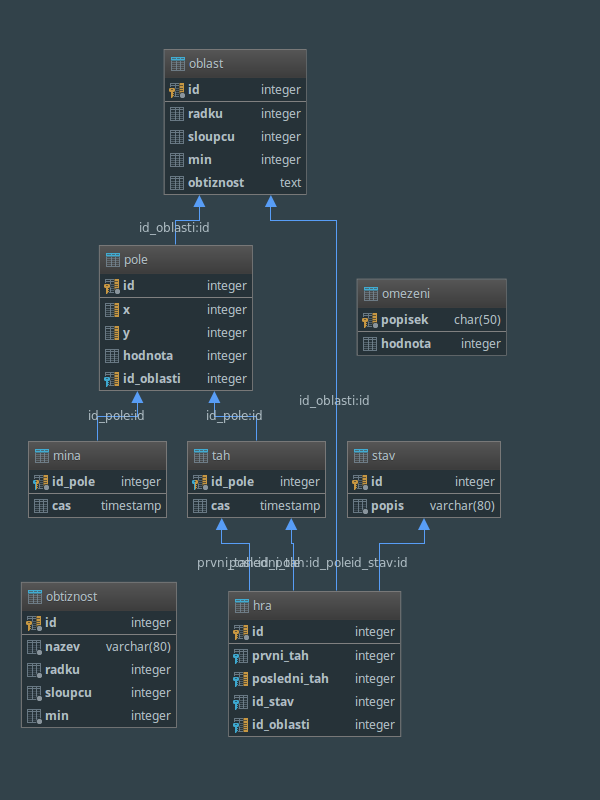
\includegraphics[width=\linewidth]{img/era.png}}
    \caption{Datový model databáze}
    \label{fig:era}
\end{center}
\end{figure}

\newpage
\section{Ukázka klientské aplikace}
\begin{figure}[!h]
\begin{center}
    \fbox{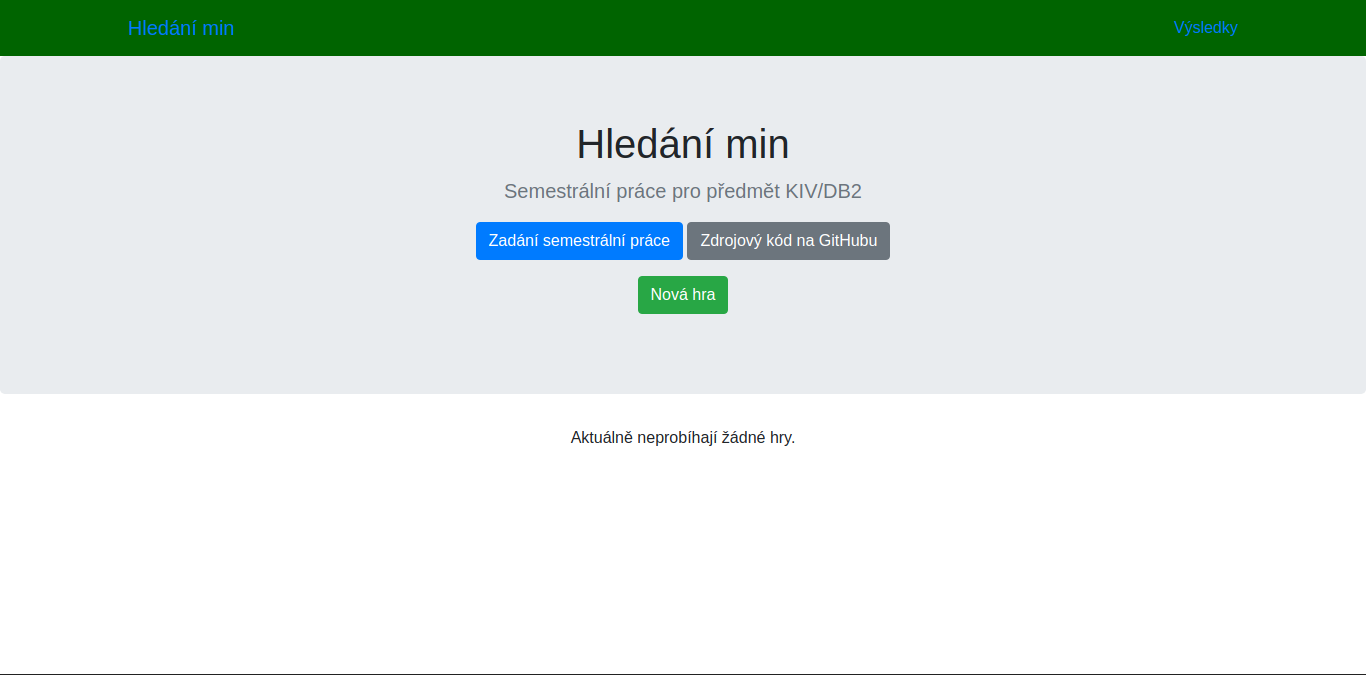
\includegraphics[width=\linewidth]{img/overview.png}}
    \caption{Hlavní stránka aplikace}
    \label{fig:overview}
\end{center}
\end{figure}

\begin{figure}[!h]
\begin{center}
    \fbox{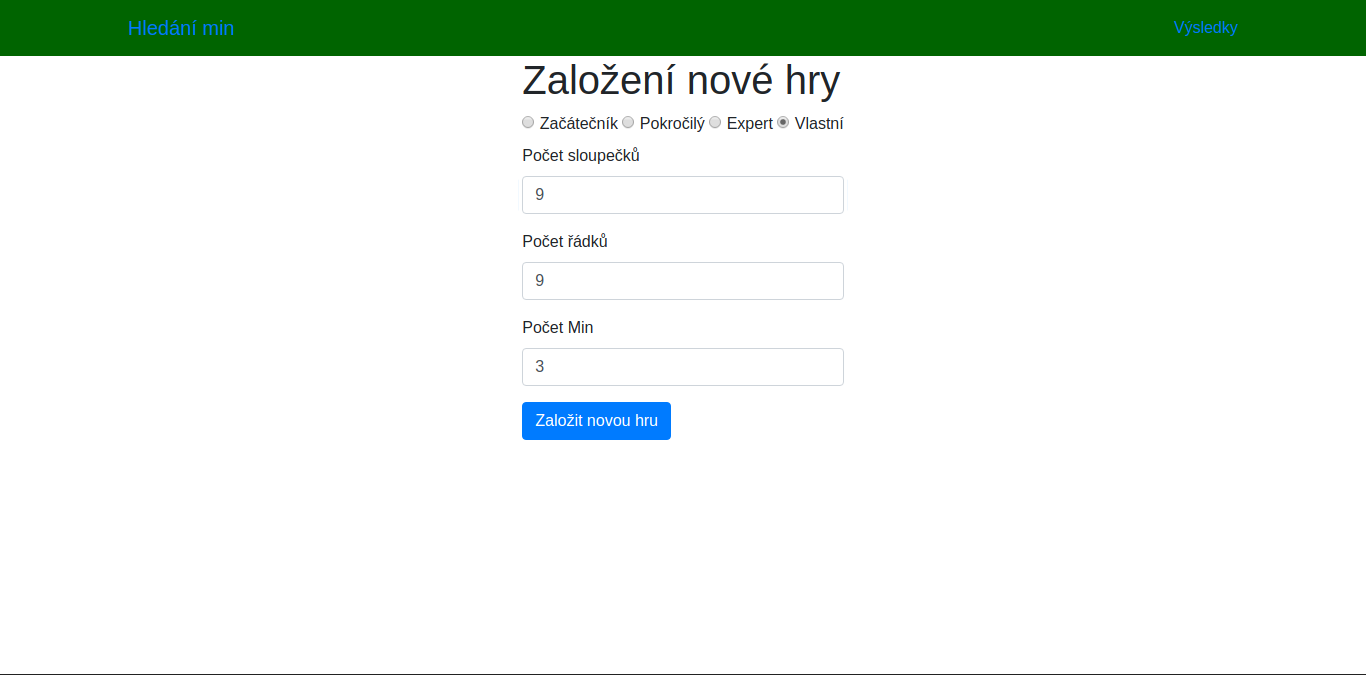
\includegraphics[width=\linewidth]{img/create_game.png}}
    \caption{Formulář pro založení nové hry}
    \label{fig:new_game}
\end{center}
\end{figure}

\begin{figure}[!h]
\begin{center}
    \fbox{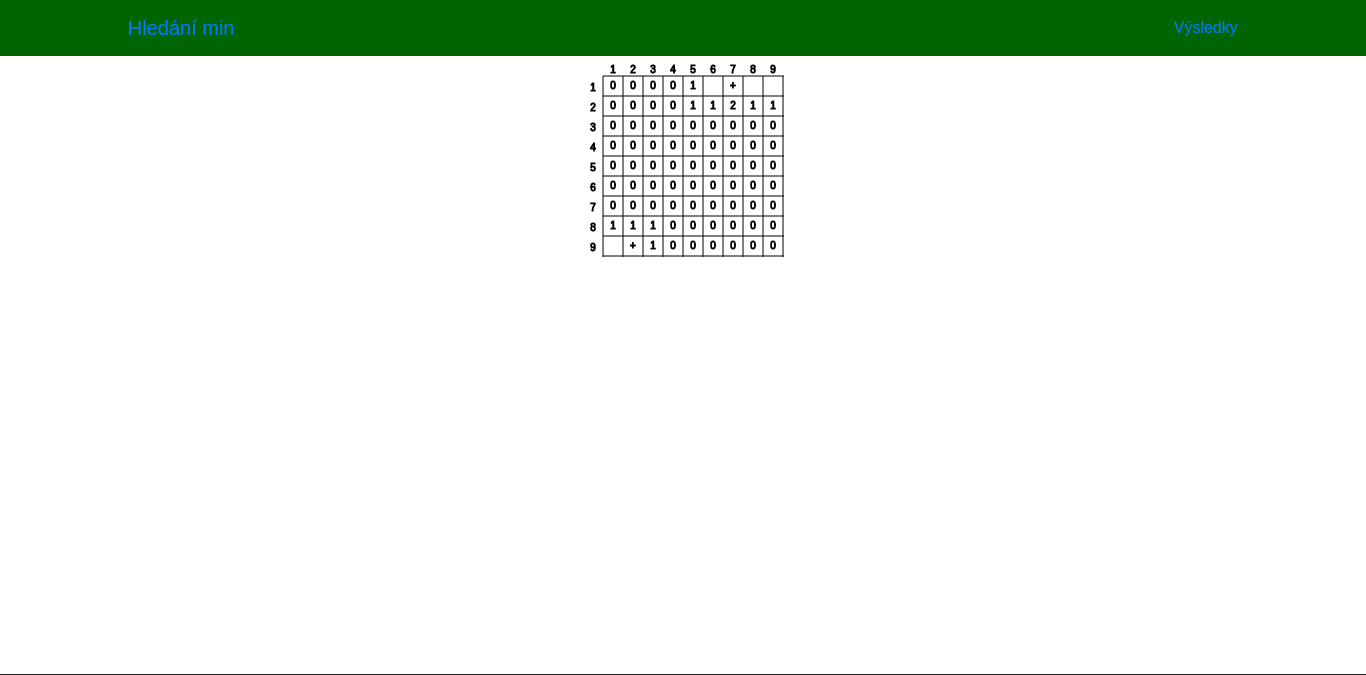
\includegraphics[width=\linewidth]{img/game.png}}
    \caption{Rozehraná hra}
    \label{fig:game}
\end{center}
\end{figure}

\begin{figure}[!h]
\begin{center}
    \fbox{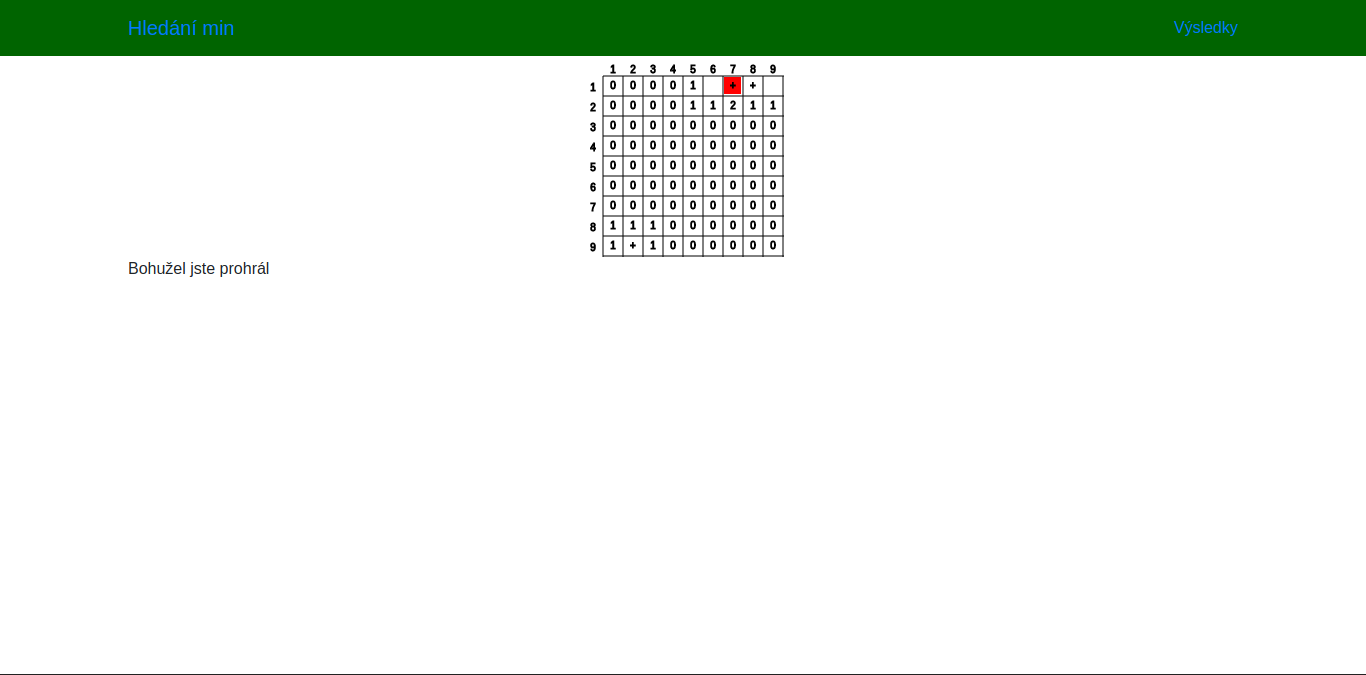
\includegraphics[width=\linewidth]{img/loose.png}}
    \caption{Prohraná hra se špatně označenými minami}
    \label{fig:loose}
\end{center}
\end{figure}

\begin{figure}[!h]
\begin{center}
    \fbox{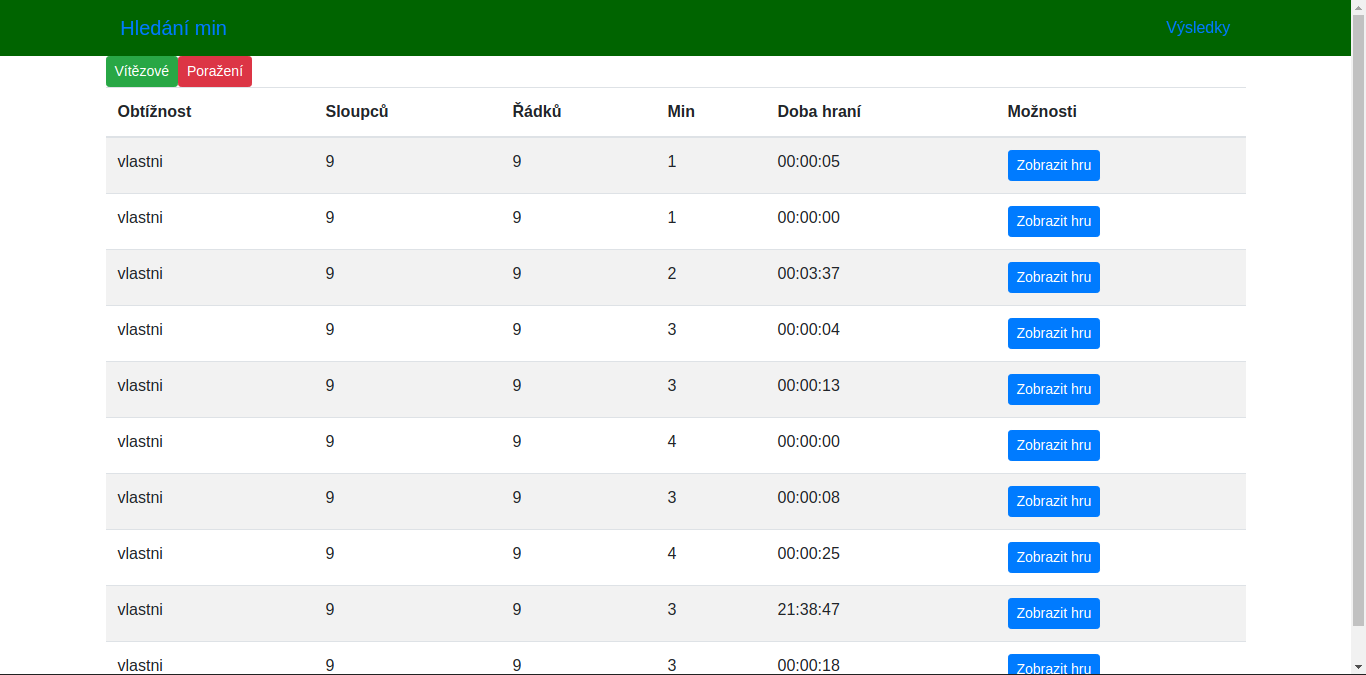
\includegraphics[width=\linewidth]{img/scoreboard.png}}
    \caption{Výsledková listina}
    \label{fig:scoreboard}
\end{center}
\end{figure}

\end{appendices}

\end{document}
